\section{Experimentación}

    En esta sección, se presentan las pruebas experimentales que se realizaron, junto con los resultados obtenidos y una discusión de los mismos.

    En primer lugar, se detallan las experiencias relacionadas con el método de \emph{PageRank} y su aplicación en el desarrollo de motores de búsqueda. Estos experimentos se hallan orientados a evaluar, por un lado, el rendimiento y la convergencia del otro, y por otra parte, la calidad de los resultados obtenidos.

    A continuación, se encuentran las pruebas relacionadas con respecto al método \emph{GeM}. Estas se encuentran focalizadas en la elaboración de \emph{rankings} para ligas futbolísticas, estudiando la factibilidad de la aplicación del algoritmo en este contexto particular, y diversas alternativas para resolver la dificultad que se presenta a la hora de tener en cuenta los empates.

    Cabe señalar que con los archivos fuente del trabajo práctico se incluye una serie de scripts en lenguaje Bash que permiten reproducir por completo los experimentos realizados, como así también los gráficos que se incluyen en este informe. Estos se encuentran dentro del directorio \texttt{exp}, y llevan los nombres \texttt{exp{i}.sh}, siendo \texttt{i} el número de experimento.

    \subsection{Experimentación con respecto a \emph{PageRank} y páginas web}

        \subsubsection{Experimento 1: Tiempo de ejecución de \emph{PageRank}}

            \subsubsection*{Presentación}
                El objetivo de este experimento fue extraer conclusiones acerca de la variación en el tiempo de cómputo requerido por el algoritmo de \emph{PageRank} para redes de diferentes tamaños, en función de la cantidad de páginas y de la cantidad de \emph{links} de las mismas.

            \subsubsection*{Metodología, datos y parámetros del experimento}
                Se realizaron pruebas para medir el rendimiento temporal según dos parámetros:
                \begin{enumerate}[label=(\alph*)]
                    \item Cantidad de páginas de la red. Se consideraron redes generadas artificialmente con las siguientes cantidades de nodos: \{200, 400, 600, 800, 1000, 1200, 1400, 1600, 1800, 2000\}, estableciendo en todas ellas la misma cantidad de enlaces, 40000, distribuidos entre las páginas de manera uniforme. Los casos de prueba se pueden generar mediante el \emph{script} \texttt{exp/exp1-a-data.sh}.

                    \item Cantidad de enlaces de la red. Se consideraron redes generadas artificialmente con una cantidad fija de 400 nodos, variando la cantidad de enlaces establecidos entre ellos, tomando los valores \{1200, 4000, 10000, 20000, 40000, 60000, 80000, 120000, 160000\}, distribuidos entre las páginas de manera uniforme. Los casos de prueba se pueden generar mediante el \emph{script} \texttt{exp/exp1-b-data.sh}.
                \end{enumerate}

                El parámetro de amortiguación $c$ se mantuvo fijo con el valor 0.85 (el utilizado normalmente por el buscador Google\cite{Brin1998}), mientras que el umbral de tolerancia para la detención del método se fijó en 0.0001.

                En cada caso, se midió el tiempo necesario para la construcción de la matriz que modela la red y para la ejecución de todas las iteraciones necesarias del método. Para realizar las mediciones se utilizaron las funciones provistas a tal efecto por la biblioteca estándar de C++. Con el fin de evitar posibles errores en las mismas, cada una se repitió 10 veces, considerando luego el promedio entre los valores obtenidos.

            \subsubsection*{Hipótesis}
            Es importante considerar en este punto la forma en que la implementación del algoritmo \emph{PageRank} aprovecha la propiedad de la matriz que modela la red ($\mat{P_1}$) de ser esparsa. Una inspección al código de dicha implementación revela que la única operación costosa que se realiza en cada iteración es  el producto entre la dicha matriz y el vector resultante de la iteración anterior. Dentro de este producto existen un ciclo que itera sobre todas las posiciones de la matriz, es decir, cuadráticamente en la cantidad de nodos, realizando un producto en cada caso, correspondiente a la multiplicación con la matriz homogénea de amortiguación ($\mat{E}$). Por otra parte, también existe un ciclo que itera sobre las posiciones no nulas de la matriz, es decir, linealmente en la cantidad de \emph{links} de la red, para realizar el producto del vector con estos coeficientes; en este caso, cada iteración requiere que se realicen dos productos.

            Teniendo en cuenta lo anterior, cabe esperar que el tiempo de ejecución dependa cuadráticamente de la cantidad de nodos de la red y linealmente, pero con una constante mayor, de la cantidad de \emph{links} de la misma.

            \subsubsection*{Resultados obtenidos}

            \subsubsection*{Discusión}

        \subsubsection{Experimento 2: Convergencia de \emph{PageRank}}

            \subsubsection*{Presentación}
            Por medio de este conjunto de pruebas experimentales, se buscó analizar la convergencia lograda por el algoritmo \emph{PageRank} en cada iteración. Como parámetro de la misma, se consideró la diferencia entre el resultado arrojado por dicha iteración y el obtenido en la inmediatamente anterior, en términos de la norma Manhattan de esta diferencia. Teniendo en cuenta que este mismo parámetro es el empleado como criterio de parada del método, se buscó extraer conclusiones sobre la relación entre la tolerancia establecida para dicho criterio y la cantidad de iteraciones necesarias para completar el algoritmo. Además, se analizó la influencia del valor del parámetro $c$ en la convergencia del método.

            \subsubsection*{Metodología, datos y parámetros del experimento}
            A los efectos del experimento, se consideraron las siguientes tres instancias de redes, una de tamaño pequeño y otras dos con cantidad de nodos mayor:
            \begin{enumerate}[label=(\alph*)]
                \item Red pequeña, formada por 50 páginas web reales y la estructura de \emph{links} determinada por las mismas, que al momento del experimento contenía 160 enlaces. La lista de sitios utilizados puede encontrarse en el archivo \texttt{exp/exp2-a-webs.txt}, y el grafo generado, en \texttt{exp/exp2-a-graph.txt}.

                \item Red mediana , formada por las páginas de la Universidad de Stanford (stanford.edu) y los enlaces entre ellas. Comprende 281903 páginas y 2312497 enlaces. Los datos, extraídos de \cite{SNAP}, fueron recopilados en 2002.

                \item Red mediana, formada por las páginas de la Universidad de Notre Dame (nd.edu) y los enlaces entre ellas. Comprende 325729 páginas y 1497134 enlaces. Los datos, extraídos de \cite{SNAP}, fueron recopilados en 1999.
            \end{enumerate}

            Está claro que el tamaño de estas redes no es comparable con el de aquellas que aparecen en el escenario de un buscador web actual (el primer índice de Google, en 1998, contenía 26 millones de páginas \cite{Brin1998}), pero se las consideró suficientes para evaluar el comportamiento del método sin incrementar desmesuradamente los tiempos de ejecución, dejando abierta la posibilidad de realizar, en el futuro, pruebas con instancias mayores.

            Sobre las tres instancias, se ejecutó el algoritmo \emph{PageRank} hasta que la diferencia entre dos iteraciones sucesivas alcanzó el umbral de tolerancia de 0.001 según la norma Manhattan, registrando el valor obtenido para la misma en cada iteración.

            En cuanto al parámetro $c$, el experimento se repitió para cada instancia con los valores \{0.85, 0.90, 0.95, 0.99\}. Se desestimaron valores menores de $c$ porque, como se argumenta en \cite{Kamvar2003}, estos producen resultados poco relevantes y aumentan demasiado la posibilidad de manipulación del método.

            \subsubsection*{Hipótesis}
            Dada la naturaleza iterativa del método, resulta razonable esperar que el ritmo de convergencia del método disminuya a medida que el resultado obtenido se acerca, de forma asintótica, al estado de equilibrio. Esto significa que el costo requerido en cantidad de iteraciones para aumentar la precisión del resultado obtenido se volverá cada vez mayor, apareciendo, en función de los requerimientos específicos del contexto de aplicación, un umbral mínimo para la tolerancia a partir del cual no valdrá la pena continuar ejecutando el método.

            En cuanto al valor de $c$, es importante recordar que valores pequeños de este parámetro determinan, a la hora de construir la matriz $\mat{P_2}$ sobre la que se aplica el algoritmo, un mayor peso relativo de la matriz de amortiguación ($\mat{E}$) con respecto a la que contiene los pesos reales de cada enlace ($\mat{P_1}$). En otras palabras, conforme disminuye el valor de $c$, cabe esperar que la matriz $\mat{P_2}$ sea más homogénea, o que se “se parezca más” a $\mat{E}$.

            Ahora bien, el vector inicial con el que se realiza la primera iteración es un vector homogéneo, que, como puede deducirse fácilmente, es el resultado esperado en caso de que la matriz de la red sea exactamente $\mat{E}$. Por lo tanto, es razonable esperar que ante valores menores de $c$, el vector inicial sea una mejor aproximación del resultado buscado, produciendo que el método converja más rápidamente.

            \subsubsection*{Resultados obtenidos}

            \subsubsection*{Discusión}

        \subsubsection{Experimento 3: Análisis cualitativo de los resultados}

            \subsubsection*{Presentación}
            Por medio de estas pruebas, se pretende realizar un estudio cualitativo de los resultados arrojados por el método \emph{PageRank}. A modo de contraste, y para realizar una evaluación comparativo, se implementó un método de clasificación alternativo más simple, denominado In-Deg. Este consiste en ordenar las páginas considerando simplemente la cantidad de \emph{links} entrantes hacia cada una de ellas. En particular, el puntaje de una página se calcula como el cociente entre la cantidad de enlaces que recibe y el total de los mismos en la red.

            \subsubsection*{Metodología, datos y parámetros del experimento}
            Para esta experiencia se construyeron artificialmente tres redes pequeñas, pensadas con el objetivo de poner de manifiesto y observar las diferencias entre los dos algoritmos planteados. Estos casos de prueba, que ilustra la Figura \ref{fig:exp3-webs}, son los siguientes:
            \begin{enumerate}[label=(\alph*)]
                \item La Web 1 cuenta con ocho nodos. Seis de los mismos (nodos 3 a 8) se encuentran enlazados de forma tal que cada uno de ellos recibe enlaces de exactamente dos de los otros. Uno de los nodos restantes (nodo 1) recibe un enlace de cada uno de estos seis. El otro (nodo 2) recibe solo un enlace de este último.
                \item La Web 2 también posee ocho nodos. Uno de ellos (nodo 1) recibe enlaces de todos los demás. Otro nodo (nodo 2) solo recibe un enlace del nodo 1. El nodo 3 recibe enlaces de los últimos cinco nodos (del 4 al 8). Estos, por su parte, no tienen enlaces entrantes.
                \item La Web 3 se compone de dos subredes no conectadas, una de 4 nodos y otra de 2 nodos. Dentro de ellas, cada nodo recibe exactamente un enlace entrante desde otro nodo.
            \end{enumerate}

            \begin{figure}[h]
                \begin{center}
                    \begin{tabular}{@{\extracolsep{2cm}} cc}
                      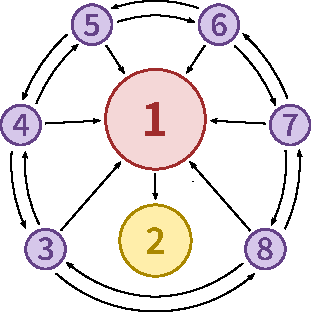
\includegraphics{imagenes/exp3-graph1.pdf} & 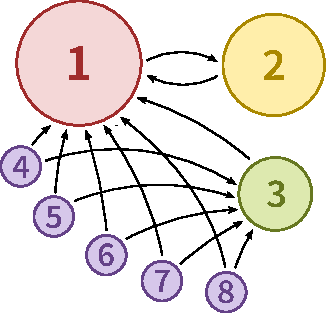
\includegraphics{imagenes/exp3-graph2.pdf} \\
                      {\small \strong{Web 1}} & {\small \strong{Web 2}} \\
                      \multicolumn{2}{c}{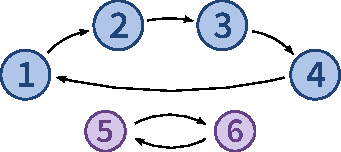
\includegraphics{imagenes/exp3-graph3.pdf}} \\
                      \multicolumn{2}{c}{{\small \strong{Web 3}}} \\
                    \end{tabular}
                \end{center}

                \caption{Redes utilizadas como datos de entrada para el Experimento 3. El tamaño con el que aparece representado cada nodo corresponde al \emph{ranking} que la hipótesis planteada prevé como resultado de \emph{PageRank}.} \label{fig:exp3-webs}
            \end{figure}

            \subsubsection*{Hipótesis}

            \subsubsection*{Resultados}

            \subsubsection*{Discusión}


% Acá sigue lo viejo

			\subsubsection*{Resultados}
				{\centering \begin{tabular}{c}
			      % 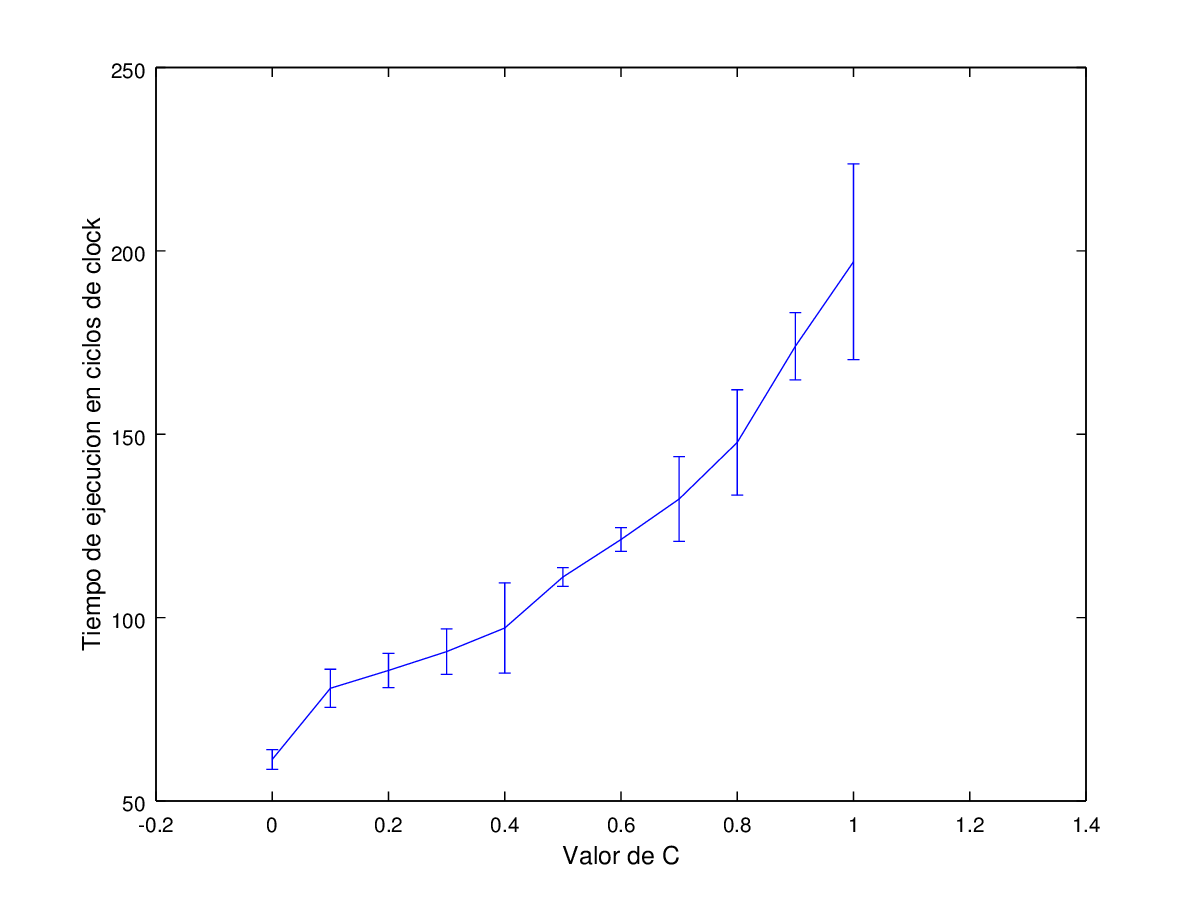
\includegraphics[width=12cm]{../../src/exp/graficos/exp1.png} \\
			    \end{tabular}}

			\subsubsection*{Discusión} 
			Como se puede observar en el experimento, a medida que aumenta el valor de c, aumenta el tiempo de ejecución. Esto se debe a que la matriz inicial no es homogénea y la que formamos a partir del c si lo es. Así, cuando la segunda toma dicha importancia, el sistema tiende más rápido a ser homogéneo y requiere menos iteraciones del ciclo para lograr una norma menor a la tolerancia deseada. 


		\subsubsection{Experimento 2}
			\subsubsection*{Presentación}
			Con este experimento se pretende observar la diferencia en el tiempo de ejecución cuando se varía la cantidad de \emph{links} en una determinada cantidad de páginas, manteniendo el valor de la tolerancia constante.
			Para ello se utilizan listas de páginas diferentes como parámetro de entrada en cada una de las ejecuciones a comparar, pero manteniendo la cantidad de las mismas. Se toma el tiempo que se demora en ejecutar el algoritmo y se lo divide por la cantidad de iteraciones realizadas. Esto permite obtener un promedio del tiempo que demora por cada una de las iteraciones del ciclo.
		
			\subsubsection*{Hipótesis} 
			Suponemos que variar la cantidad de \emph{links} altera más el tiempo de ejecución que variar la cantidad de páginas sin que estén relacionadas entre ellas. Esto se debe a que, dada la forma en la que está implementado el algoritmo, sacando provecho del hecho de que la matriz es esparsa, agregar entradas a la matriz de adyacencia tendrá un mayor impacto sobre la cantidad de operaciones a realizar. Por lo tanto, se espera observar que el tiempo de ejecución aumente a medida que la cantidad de relaciones entre páginas sea mayor.

			\subsubsection*{Datos de entrada} 		
			Para este experimento se toman 50 páginas. La cantidad de \emph{links} entre ellas varía, tomando los valores \texttt{4, 32, 70, 105, 130, 160}. Estos valores fueron elegidos a modo de análisis. Para generarlos se creó una red a partir de diferentes páginas web interconectadas entre sí. Luego se borraron algunas páginas, eliminando una determinada cantidad de \emph{links}, y se agregaron nuevas páginas desconectadas totalmente de las ya existentes. De esta forma, no se disminuyó la cantidad de páginas pero sí la de \emph{links}. Además el valor de $c$ es \texttt{0.85} y el valor de la tolerancia es \texttt{0.00001}. El valor de $c$ y de la tolerancia fueron elegidos arbitrariamente, procurando que los casos de prueba no fueran excesivamente grandes para no prolongar innecesariamente la duración de las pruebas. 
			
			\subsubsection*{Resultados}
				{\centering \begin{tabular}{c}
			      % 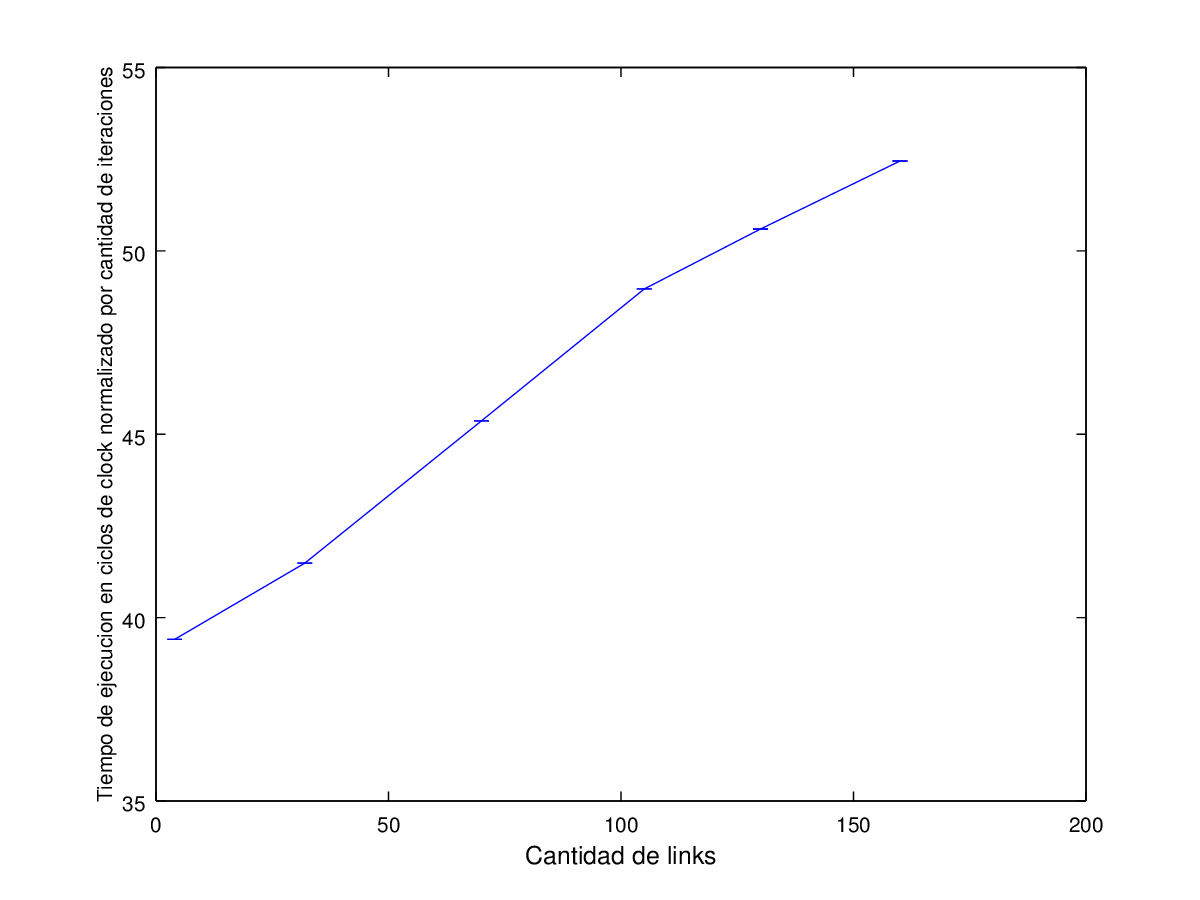
\includegraphics[width=12cm]{../../src/exp/graficos/exp2.png} \\
			    \end{tabular}}


			\subsubsection*{Discusión}
			Como se puede observar en el gráfico, a medida que aumentan las relaciones entre las páginas el tiempo de ejecución es mayor.  

		\subsubsection{Experimento 3}
			\subsubsection*{Presentación}
			En este experimento también se observa la diferencia en el tiempo de ejecución, pero comparando igual cantidad de páginas y relaciones entre las mismas y variando el valor de la tolerancia.
			Para ello se toma como parámetro de entrada en cada una de las ejecuciones una misma lista de páginas y se incrementa el valor de la tolerancia.

			\subsubsection*{Hipótesis} 
			Creemos que cuanto mayor sea la tolerancia, menor será el tiempo de ejecución del algoritmo. Esto se debe a que el algoritmo termina cuando la diferencia Manhattan es menor que la tolerancia. Entonces cuanto más grande sea el valor de la tolerancia, más rápido se cumplirá la condición para salir del ciclo y menos tardará en ejecutarse el algoritmo. Suponemos que para los valore mas chicos de tolerancia el tiempo de ejecución será altamente mayor que para valores de tolerancia cercanos a 1. Es decir, el crecimiento será exponenecial a medida que disminuimos el valor de la tolerancia.

			\subsubsection*{Datos de entrada} 
			Se toman 13 páginas con 16 \emph{links}. Además la tolerancia toma los siguientes valores: \texttt{0.000001, 0.000005, 0.00001, 0.00005, 0.0001, 0.0005, 0.001, 0.005, 0.01, 0.1, 0.3, 0.5, 0.7}. El parámetro $c$ es igual a \texttt{0.85}. El valor de $c$ y la cantidad de páginas fueron elegidos arbitrariamente, procurando que los casos de prueba no fueran excesivamente grandes para no prolongar innecesariamente la duración de las pruebas. Los valores de la tolerancia fueron tomados a modo de análisis teniendo en cuenta que el objetivo del experimento. 

			\subsubsection*{Resultados}
				{\centering \begin{tabular}{c}
			      % 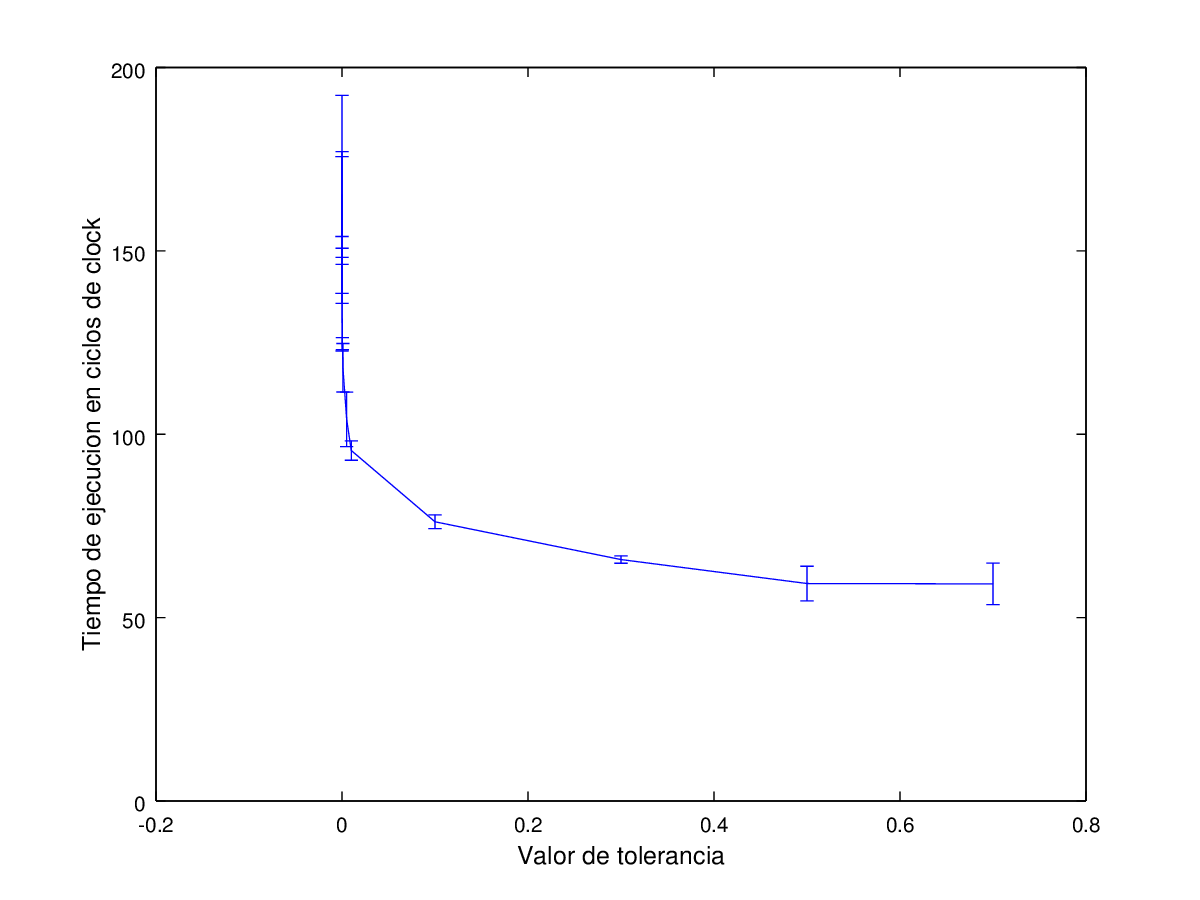
\includegraphics[width=12cm]{../../src/exp/graficos/exp3.png} \\
			    \end{tabular}}

			\subsubsection*{Discusión}
			Como se puede ver en el gráfico, al aumentar la tolerancia disminuye el tiempo de ejecución linealmente. Al estar en escala logaritmica, esto quiere decir que la función decrece de forma exponencial. Para valores de tolerancia cercanos a 1, la cantidad de iteraciones a realizar es notoriamente menor que para valores de tolerancia cercanos a 0. Esto sucede ya que el método converge cada vez mas lento, entonces cuando la tolerancia toma valores muy chicos las ultimas iteraciones modifican muy poco el vector por lo que se requieren más iteraciones para acercarse al resultado.
			Además se puede observar que hasta el valor de tolerancia 0.01 la variación en tiempo de ejecución dependiendo del valor de la tolerancia es mínimo. Cuando ese valor es menor que 0.01 el tiempo de ejecución se incrementa notoriamente. Dejamos a experimentos futuros ver cuál es el valor en el que el tiempo de ejecución es muy grande. En este sentido, se pudo confirmar la hipótesis.   

	\subsubsection{Experimento 4}
		\subsubsection*{Presentación}
		Otra de las pruebas consiste en comparar los \emph{rankings} formados al ejecutar los algoritmos de \emph{PageRank} y el de \textsc{In-deg}. Primero se analiza una lista de páginas de entrada en la que una de ellas sea apuntada por el resto (Web 1). 

		Luego se realiza la comparación con una lista en la que hayan dos páginas (a las que llamaremos página 1 y página 3) que sean apuntadas por varias paginas. Además, la página 3 tendrá un link a la 1. También se cuenta con otra (a la que llamaremos página 2) que apunta y es apuntada por la página 1, tal como se muestra en el siguiente esquema (Web 2):

			\begin{figure}[h]

				\begin{center}
					\begin{tabular}{@{\extracolsep{2cm}} cc}
				      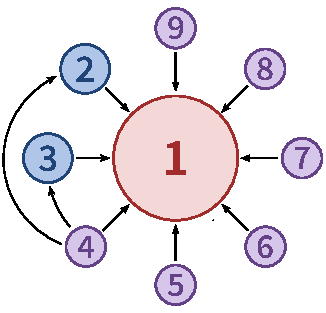
\includegraphics{imagenes/exp4-graph1.pdf} & 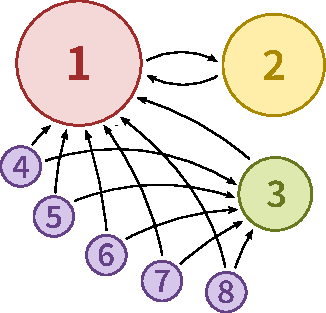
\includegraphics{imagenes/exp4-graph2.pdf} \\
				      {\small \strong{Web 1}} & {\small \strong{Web 2}}
				    \end{tabular}
			    \end{center}

		    	\caption{Redes utilizadas como datos de entrada para el Experimento 4} \label{fig:exp4-webs}

		    \end{figure}

			\subsubsection*{Hipótesis} 
			En el primero, suponemos que los \emph{rankings} obtenidos en ambos casos serán iguales ya que existe una sola página principal y el resto tiene igual cantidad de relaciones. Por otro lado, en el segundo notaremos diferencias. Llamaremos enlace fuerte a aquel que va de una página que es apuntada por muchas otras hacia otra página. El método \emph{PageRank} tiene en cuenta cuál es el peso de los \emph{links} que apuntan a las distintas páginas. En el caso de \textsc{In-deg}, solo se utiliza como información la cantidad de enlaces que llegan a cada una de las distintas páginas.

			En el experimento, si consideramos el método \emph{PageRank}, la página 1 quedará en primer lugar, ya que es la que recibe más \emph{links} a la misma, pero en segundo lugar quedará la página 2. Esto se debe a que el enlace de la 1 a la 2 es un enlace muy fuerte. En el caso de \textsc{In-deg}, esto no sucede ya que este método solo toma en cuenta que existe un único link hacia la página 2. Por lo tanto en \emph{PageRank} las posiciones serán 1-2-3 y luego el resto. En \textsc{In-deg} tendremos primero a la página 1 seguida de la 3, luego la 2 y finalmente el resto.

			\subsubsection*{Datos de entrada}
			Para la Web 1, se tomaron 9 páginas con 10 \emph{links}. Para la Web 2, se tomaron 8 páginas con 13 \emph{links}.  

			El valor de $c$ es \texttt{0.85} y el valor de tolerancia es \texttt{0.00001}. 
			 		
			\subsubsection*{Resultados}

			   \begin{center}
	      			\begin{tabular}{c|c|c} 
			      		\hline
			  				\multicolumn{3}{c}{\emph{Ranking} Web 1 - \emph{PageRank}} \\
			 			\hline
	        			Posición & Nodo & Puntaje \\ \hline
	         			1 & 1 & 0.473848 \\
	        			2 & 8 & 0.078821 \\
	        			3 & 9 & 0.078821 \\
	        			4 & 2 & 0.061418 \\
	        			5 & 3 & 0.061418 \\
	        			6 & 4 & 0.061418 \\
	        			7 & 5 & 0.061418 \\
	        			8 & 6 & 0.061418 \\
	        			9 & 7 & 0.061418 
	      			\end{tabular} 

	      			\begin{tabular}{c|c|c}
			      		\hline
			  				\multicolumn{3}{c}{\emph{Ranking} Web 1 - \textsc{In-deg}} \\
			 			\hline
	        			Posición & Nodo & Puntaje \\ \hline
	         			1 & 1 & 0.8 \\
	        			2 & 8 & 0.1 \\
	        			3 & 9 & 0.1 \\
	        			4 & 2 & 0 \\
	        			5 & 3 & 0 \\
	        			6 & 4 & 0 \\
	        			7 & 5 & 0 \\
	        			8 & 6 & 0 \\
	        			9 & 7 & 0 
	      			\end{tabular}

	      			\begin{tabular}{c|c|c}
			      		\hline
			  				\multicolumn{3}{c}{\emph{Ranking} Web 2 - \emph{PageRank}} \\
			 			\hline
	        			Posición & Nodo & Puntaje \\ \hline
	         			1 & 1 & 0.448059 \\
	        			2 & 2 & 0.448059 \\
	        			3 & 3 & 0.058594 \\
	        			4 & 4 & 0.058594 \\
	        			5 & 5 & 0.018750 \\
	        			6 & 6 & 0.018750 \\
	        			7 & 7 & 0.018750 \\
	        			8 & 8 & 0.018750
	      			\end{tabular}
	    		
	      			\begin{tabular}{c|c|c}
			      		\hline
			  				\multicolumn{3}{c}{\emph{Ranking} Web 2 - \textsc{In-deg}} \\
			 			\hline
	        			Posición & Nodo & Puntaje \\ \hline
	         			1 & 1 & 0.538462 \\
	        			2 & 3 & 0.384615 \\
	        			3 & 2 & 0.076923 \\
	        			4 & 4 & 0 \\
	        			5 & 5 & 0 \\
	        			6 & 6 & 0 \\
	        			7 & 7 & 0 \\
	        			8 & 8 & 0 \\
	      			\end{tabular}
	    	\end{center}

			\subsubsection*{Discusión} 
			Como podemos ver en los \emph{rankings} del primer análisis en ambos casos quedan iguales. En cambio, en el segundo observamos variaciones, ya que en la lista de entrada el peso de todos los enlaces no es el mismo, es decir, hay enlaces más fuertes que otros. A diferencia de \emph{PageRank}, el método \textsc{In-deg} no tiene en cuenta esta propiedad. Por lo tanto, si en las páginas de entrada todos los \emph{links} tienen igual fuerza, el resultado obtenido por ambos métodos no difiere. 


	\subsection{\emph{GeM} y ligas deportivas}
		
		\subsubsection{Experimento 1}
		\subsubsection*{Presentación}
		En este experimento se verá la diferencia entre los métodos de \emph{GeM} y el de la \acr{AFA} para determinar el \emph{ranking} de una liga deportiva. Para ello se tomará como parámetro de entrada una tabla con los partidos, sus respectivas fechas, y sus resultados. En la misma, deberá existir un equipo que ocupe una de las primaras posiciones en la tabla de \emph{rankings} que haya perdido contra otro que ocupa una de las últimas. Observaremos la diferencia entre el \emph{ranking} generado por cada uno de los métodos.

			\subsubsection*{Hipótesis} 
			Cuando se juega un partido entre dos equipos, en el método de \emph{GeM} se tendrá en cuenta que tan fuerte son los equipos involucrados y cual fue la diferencia de goles en el partido. En cambio, en el método de la \acr{AFA} el ganador recibirá 3 puntos sin importar los resultados ni las posiciones que los mismos tenían hasta el momento. Esto puede generar diferencias en el \emph{ranking} ya que cada método considera distinta información para determinar las nuevas posiciones. 
			
			Por otro lado, si un equipo que se encuentra en las últimas posiciones de la tabla juega contra uno que está en las primeras y gana, para el método de la \acr{AFA} es exactamente igual que haya jugado con cualquier otro. Para \emph{GeM}, al tener en cuenta que tan fuertes son los equipos, esto generará que el nuevo vencedor quede en una mejor posición en la tabla. Así, en este método, entre dos fechas se pueden generar saltos, es decir, un equipo puede pasar de tener una muy mala posición en la tabla a estar dentro de los mejores solo por haber ganado un partido contra un equipo fuerte. En el método de la \acr{AFA} no pasa ya que sólo se le sumarán 3 puntos al equipo triunfador.		

			\subsubsection*{Datos de entrada} 
				Resultados del Torneo de Primera División del Fútbol Argentino hasta la Fecha 23. El valor de $c$ es \texttt{0.85} y el valor de tolerancia es \texttt{0.00001}. Se eligió el valor de c y el de la tolerancia arbitrariamente, procurando que los casos de prueba no fueran excesivamente grandes para no prolongar innecesariamente la duración de las pruebas. 
. 

			\subsubsection*{Resultados}

				\begin{center}
	      			\begin{tabular}{|c|c|c|} 
			      		\hline
			  				\multicolumn{3}{c}{\emph{Ranking} Liga Deportiva - \emph{GeM}} \\
			 			\hline
	        			Posición & Equipo & Puntaje \\ \hline
	         			1 & Boca Juniors & 0.080913 \\
	        			2 & Aldosivi & 0.069879 \\
	        			3 & River Plate & 0.069065 \\
	        			4 & San Lorenzo & 0.058309 \\
	        			5 & San Martín (SJ) & 0.051788 \\
	        			6 & Racing Club & 0.051674 \\
	        			7 & Rosario Central & 0.046326 \\
	        			8 & Quilmes & 0.045206 \\
	        			9 & Newell's Old Boys & 0.043581 \\
	        			10 & Vélez Sarsfield & 0.039828 \\
	        			11 & Gimnasia y Esgrima (LP) & 0.035738 \\
	        			12 & Estudiantes (LP) & 0.034629 \\
	        			13 & Belgrano & 0.033908 \\
	        			14 & Banfield & 0.032996 \\
	        			15 & Unión & 0.028015 \\
	        			16 & Defensa y Justicia & 0.027041 \\
	        			17 & Lanús & 0.026036 \\
	   					18 & Independiente & 0.023666 \\
	   					19 & Tigre & 0.023078 \\
	   					20 & Sarmiento & 0.022266 \\
	   					21 & Olimpo & 0.021956 \\
	   					22 & Crucero del Norte & 0.021713 \\
	  					23 & Arsenal & 0.018678 \\
	   					24 & Argentinos Juniors & 0.017951 \\
	   					25 & Tempreley & 0.017670 \\
	   					26 & Huracán & 0.013740 \\
	   					27 & Godoy Cruz & 0.013541 \\
	   					28 & Atlético de Rafaela & 0.011738 \\
	   					29 & Colón & 0.011141 \\
	   					30 & Nueva Chicago & 0.007928 

	      			\end{tabular} 
	      			    \begin{tabular}{|c|c|c|} 
			      		\hline
			  				\multicolumn{3}{c}{\emph{Ranking} Liga Deportiva - \acr{AFA}} \\
			 			\hline
	        			Posición & Equipo & Puntaje \\ \hline
						    1 & San Lorenzo & 0.054289 \\
						    2 & Boca Juniors & 0.053203 \\
						    3 & Racing Club & 0.049946 \\
						    4 & Rosario Central & 0.048860 \\
						    5 & River Plate & 0.047774 \\
						    6 & Independiente & 0.041260 \\
						    7 & Belgrano & 0.041260 \\
						    8 & Estudiantes (LP) & 0.041260 \\
						    9 & Tigre & 0.040174 \\
						   10 & Banfield & 0.040174 \\
						   11 & Lanús & 0.039088 \\
						   12 & Gimnasia y Esgrima (LP) & 0.038002 \\
						   13 & Quilmes & 0.034745 \\
						   14 & San Martín (SJ) & 0.034745 \\
						   15 & Unión & 0.033659 \\
						   16 & Tempreley & 0.030402 \\
						   17 & Argentinos Juniors & 0.028230 \\
						   18 & Newell's Old Boys & 0.028230 \\
						   19 & Aldosivi & 0.028230 \\
						   20 & Vélez Sarsfield & 0.027144 \\
						   21 & Defensa y Justicia & 0.026059 \\
						   22 & Sarmiento & 0.026059 \\
						   23 & Olimpo & 0.024973 \\
						   24 & Colón & 0.024973 \\
						   25 & Godoy Cruz & 0.023887 \\
						   26 & Huracán & 0.022801 \\
						   27 & Atlético de Rafaela & 0.021716 \\
						   28 & Arsenal & 0.018458 \\
						   29 & Nueva Chicago & 0.015201 \\
						   30 & Crucero del Norte & 0.015201 \\

	      			\end{tabular} 
	      	\end{center}

			\subsubsection*{Discusión}


			Como podemos ver en las tablas de \emph{rankings}, los órdenes no son exactamente iguales. Por ejemplo, mirando el equipo 1 (Aldosivi), en el \emph{ranking} de la \acr{AFA} se encuentra en la posición 20 y cuando usamos el método de \emph{GeM} éste está en la posición 2. Esto se debe a que Aldosivi le ganó tanto al equipo 24 (San Lorenzo) como al 7 (Boca Juniors), que se encontraban primero y segundo en la tabla de posiciones de la \acr{AFA}, respectivamente. Por esto, en \emph{GeM} sube muchas posiciones mientras que con la \acr{AFA} sólo se le otorgan 3 puntos por cada uno de los dos partidos.

